\documentclass[parskip,a4paper,12pt]{article}
\input{preambulo}
\newcommand{\Practica}{Práctica P4}
\newcommand{\Grupo}{Grupo X} %  
\newcommand{\NombreUNO}{Apellidos1, Nombre1}
\newcommand{\NombreDOS}{Apellidos2, Nombre2} %\shortstack{Apellidos, Nombre\\Apellidos, Nombre}
\def\portada{1} % 1 ó 2 ó 3
\graphicspath{{graficosP4/}}
\newcommand{\fila}{}
\usepackage{ifthen}
%%%%%%%%%%%%%%%%%%%%%%%%%%%%%%%%%%%%%%%%%%%%%%%%%%%%%%
\begin{document}
\setcounter{tcb@cnt@enunciado}{28}
\renewcommand{\tablename}{Tabla}
\addtocounter{page}{-1}
\startcontents[sections]
\thispagestyle{empty}
\input{portada}
\clearpage
\printmyminitoc


\section{P4\_1: Filtro compensador del CIC}
\subsection{Descripción del módulo \emph{comp\_cic}}
%%%%%%%%%%%%%%%%%%%%%%%%%
\begin{enunciado}{}{}%
Breve explicación del bloque implementado indicando su funcionalidad y estructura interna. Se puede añadir (de apoyo a la explicación) una figura con el diagrama de bloques interno del módulo \emph{comp\_cic}.
\end{enunciado}
%%%%%%%%%%%%%%%%%%%%%%%%%%%%%%%%%%%%%%%%%%%%%%%%%%%%%%%%%%%%%%%%%%%%%%%%%

%  .d8888b.   d888   % 
% d88P  Y88b d8888   % 
% 888    888   888   % 
% 888    888   888   % 
% 888    888   888   % 
% 888    888   888   % 
% Y88b  d88P   888   % 
%  "Y8888P"  8888888 % 
%%%%%%%%%%%%%%%%%%%%%%%%%
\subsection{Análisis de la cuantificación de la ruta de datos}
%%%%%%%%%%%%%%%%%%%%%%%%%
\begin{enunciado}{}{}%
Rellene la tabla indicando la cuantificación obtenida para los coeficientes, el crecimiento de la ruta de datos (Ng) y la cuantificación para obtener la salida con precisión completa. Explique cómo ha obtenido estos valores.
\end{enunciado}
% TABLA CUANTIFICACION (3 COLUMNAS) %%%%%%%%%%%%%%%%%%%%%%%%
\input{tabla_3col}
% Definir los anchos de columna de la tabla
\def\colUNO{8cm}
\def\colDOS{3cm}
\def\colTRES{3cm}
    
\begin{table}[H]
\begin{center}
   \caption{Cuantificación interna }
    \label{tab:interfaz}
\gdef\cabecera{\fila{}{PARÁMETRO}{VALOR}}
\noindent\begin{mitabla}
\fila {Coeficientes}{[Wcoef, Fcoef]}{}
\fila {Crecimiento ruta de datos }{Ng}{}
\fila{Salida precisión completa}{[Wout, Fout]}{}
\fila{Salida precisión recortada}{[Wout, Fout]}{S[18, 15]}


\end{mitabla}

\end{center}

\end{table}

%%%%%%%%%%%%%%%%%%%%%%%%%
%  .d8888b.   .d8888b.  % 
% d88P  Y88b d88P  Y88b % 
% 888    888        888 % 
% 888    888      .d88P % 
% 888    888  .od888P"  % 
% 888    888 d88P"      % 
% Y88b  d88P 888"       % 
%  "Y8888P"  888888888  % 
%%%%%%%%%%%%%%%%%%%%%%%%%
\subsection{Interfaz}
%%%%%%%%%%%%%%%%%%%%%%%%%
\begin{enunciado}{}{}%
Incluir las tablas en las que se defina el interfaz de todos los módulos implementados, sus formatos y sus parámetros. 
\end{enunciado}
%%%%%%%%%%%%%%%%%%%%%%%%%%%%%%%%%%%%%%%%%%%%%%%%%%%%%%%%%%%%%%%%%%%%%%%%%


% TABLA DEL INTERFAZ (4 COLUMNAS) %%%%%%%%%%%%%%%%%%%%%%%%
\input{tabla_4col}
% Definir los anchos de columna de la tabla
\def\colUNO{2cm}
\def\colDOS{1cm}
\def\colTRES{2.0cm}
\def\colCUATRO{8cm}

\begin{table}[H]
    \caption{Interfaz del módulo  \emph{comp\_cic\_reg\_mux}}
    \label{tab:interfaz}
\gdef\cabecera{\fila{NOMBRE}{TIPO}{FORMATO}{DESCRIPCIÓN}}
\noindent\begin{mitabla}
% COMPLETAR FILAS. AÑADA LAS QUE NECESITE
\fila{}{}{}{} 
\fila{}{}{}{} 
\fila{}{}{}{} 
\fila{}{}{}{} 
\fila{}{}{}{} 
\fila{}{}{}{} 
\fila{}{}{}{} 
\fila{}{}{}{} 
\fila{}{}{}{} 
\fila{}{}{}{} 
\end{mitabla}
\end{table}

\begin{table}[H]
    \caption{Interfaz del módulo  \emph{comp\_cic\_mult\_add}}
    \label{tab:interfaz}
\gdef\cabecera{\fila{NOMBRE}{TIPO}{FORMATO}{DESCRIPCIÓN}}
\noindent\begin{mitabla}
% COMPLETAR FILAS. AÑADA LAS QUE NECESITE
\fila{}{}{}{} 
\fila{}{}{}{} 
\fila{}{}{}{} 
\fila{}{}{}{} 
\fila{}{}{}{} 
\fila{}{}{}{} 
\fila{}{}{}{} 
\fila{}{}{}{} 
\fila{}{}{}{} 
\fila{}{}{}{} 
\end{mitabla}
\end{table}

\begin{table}[H]
    \caption{Interfaz del módulo  \emph{comp\_cic\_rom}}
    \label{tab:interfaz}
\gdef\cabecera{\fila{NOMBRE}{TIPO}{FORMATO}{DESCRIPCIÓN}}
\noindent\begin{mitabla}
% COMPLETAR FILAS. AÑADA LAS QUE NECESITE
\fila{}{}{}{} 
\fila{}{}{}{} 
\fila{}{}{}{} 
\fila{}{}{}{} 
\fila{}{}{}{} 
\fila{}{}{}{} 
\fila{}{}{}{} 
\fila{}{}{}{} 
\fila{}{}{}{} 
\fila{}{}{}{} 
\end{mitabla}
\end{table}

\begin{table}[H]
    \caption{Interfaz del módulo  \emph{comp\_cic\_control}}
    \label{tab:interfaz}
\gdef\cabecera{\fila{NOMBRE}{TIPO}{FORMATO}{DESCRIPCIÓN}}
\noindent\begin{mitabla}
% COMPLETAR FILAS. AÑADA LAS QUE NECESITE
\fila{}{}{}{} 
\fila{}{}{}{} 
\fila{}{}{}{} 
\fila{}{}{}{} 
\fila{}{}{}{} 
\fila{}{}{}{} 
\fila{}{}{}{} 
\fila{}{}{}{} 
\fila{}{}{}{} 
\fila{}{}{}{} 
\end{mitabla}
\end{table}

\begin{table}[H]
    \caption{Interfaz del módulo  \emph{comp\_cic}}
    \label{tab:interfaz}
\gdef\cabecera{\fila{NOMBRE}{TIPO}{FORMATO}{DESCRIPCIÓN}}
\noindent\begin{mitabla}
% COMPLETAR FILAS. AÑADA LAS QUE NECESITE
\fila{}{}{}{} 
\fila{}{}{}{} 
\fila{}{}{}{} 
\fila{}{}{}{} 
\fila{}{}{}{} 
\fila{}{}{}{} 
\fila{}{}{}{} 
\fila{}{}{}{} 
\fila{}{}{}{} 
\fila{}{}{}{} 
\end{mitabla}
\end{table}
%%%%%%%%%%%%%%%%%%%%%%%%% 
%  .d8888b.   .d8888b.  % 
% d88P  Y88b d88P  Y88b % 
% 888    888      .d88P % 
% 888    888     8888"  % 
% 888    888      "Y8b. % 
% 888    888 888    888 % 
% Y88b  d88P Y88b  d88P % 
%  "Y8888P"   "Y8888P"  % 
%%%%%%%%%%%%%%%%%%%%%%%%% 
\subsection{Diseño de la Máquina de Estados}
%%%%%%%%%%%%%%%%%%%%%%%%%
\begin{enunciado}{}{}%
Incluir una breve descripción del comportamiento de la máquina de estados diseñada en el módulo \emph{comp\_cic\_control}. Dibujar el diagrama de estados de manera que incluya las señales que provocan las transiciones entre estados. Para documentar las salidas que se activan en cada estado debe incluirlas en una tabla.
\end{enunciado}
% EJEMPLO DE DIAGRAMA DE ESTADOS
\begin{figure}[h]
\centering
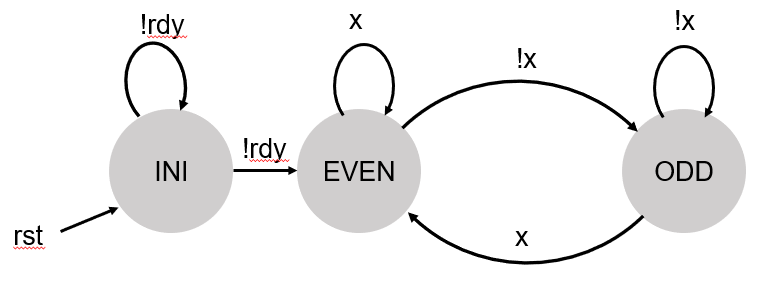
\includegraphics[width=8cm]{graficosP4/Ejem_FSM.png}
\caption{Digrama de estados de \emph{comp\_cic\_control}} 
\label{fig:photo_setup2}
\end{figure}

% EJEMPLO DE TABLA DE SALIDAS
% TABLA DEL INTERFAZ (4 COLUMNAS) %%%%%%%%%%%%%%%%%%%%%%%%
\input{tabla_2col}
% Definir los anchos de columna de la tabla
\def\colUNO{3cm}
\def\colDOS{12cm}
\begin{table}[H]
    \caption{Tabla de salidas de COMP\_CIC\_CONTROL}
    \label{tab:FSM1}
\gdef\cabecera{\fila{ESTADO}{SALIDAS}}
\noindent\begin{mitabla}
 COMPLETAR FILAS
\fila{INI}{a=0; b=0;} 
\fila{EVEN}{a=1; b=0;} 
\fila{ODD}{a=0; b=1;} 
\end{mitabla}
\end{table}
%%%%%%%%%%%%%%%%%%%%%%%%%%%%%%%%%%%%%%%%%%%%%%%%%%%%%%%%%%%%%%%%%%%%%%%%%

%%%%%%%%%%%%%%%%%%%%%%%%%
%  .d8888b.      d8888  % 
% d88P  Y88b    d8P888  % 
% 888    888   d8P 888  % 
% 888    888  d8P  888  % 
% 888    888 d88   888  % 
% 888    888 8888888888 % 
% Y88b  d88P       888  % 
%  "Y8888P"        888  % 
%%%%%%%%%%%%%%%%%%%%%%%%%


\subsection{Recursos hardware}
%%%%%%%%%%%%%%%%%%%%%%%%%
\begin{enunciado}{}{}%
El objetivo de esta sección es que el alumno sea capaz de identificar si los recursos obtenidos en la implementación son coherentes con los esperables para el circuito realizado.

Se deberán incluir las siguientes partes: 
\begin{itemize}
\item \textbf{Estimación de recursos:} Un breve desglose de la estimación de recursos  del dispositivo FPGA que se requieren para implementar el módulo, indicando la cantidad de recursos asignados a cada bloque de su diseño. El resultado final se mostrará en una tabla. En esta práctica solo hay que indicar el número de LEs en modo aritmético, los FFs y los multiplicadores embebidos. 

\item \textbf{Resultados obtenidos:} Una captura del resumen de recursos obtenidos con la herramienta Quartus tras la etapa de emplazamiento y rutado (Fitter), que se muestra en el report ``Resource Usage Summary''.  

\item \textbf{Análisis del resultado:} Un breve análisis de si los resultados obtenidos son coherentes con la estimación de recursos realizada. El análisis se realizará en base a la comparación entre lo estimado y obtenido en Quartus. Si hay muchas discrepancias con los recursos obtenidos, indicar razonadamente las causas de dicha discrepancia.
\end{itemize}

\end{enunciado}
%%%%%%%%%%%%%%%%%%%%%%%%%%%%%%%%%%%%%%%%%%%%%%%%%%%%%%%%%%%%%%%%%%%%%%%%%
A continuación se muestra la tabla con el resumen de los recursos:

% TABLA DEL INTERFAZ %%%%%%%%%%%%%%%%%%%%%%%%
\input{tabla_3col}
% Definir los anchos de columna de la tabla
\def\colUNO{5.5 cm}
\def\colDOS{5 cm}
\def\colTRES{5 cm}
%\def\colCUATRO{10cm}

\begin{table}[H]
\centering
    \caption{Recursos hardware}
    \label{tab:recursos_HW}
\gdef\cabecera{\fila{RECURSO}{NÚMERO OBTENIDO}{NÚMERO ESTIMADO}}
\noindent\begin{mitabla}
% COMPLETAR FILAS
\fila{FFs}{}{}  
\fila{LEs-aritméticos}{}{}  
\fila{Multiplicadores embebidos}{}{}  
\end{mitabla}
\end{table}

A continuación se muestra la captura realizada de los recursos obtenidos tras la etapa de emplazamiento y rutado 
(\textit{Fitter}) en el ``\textit{ Resource Usage Summary}'': 

\begin{figure}
  \begin{center}
 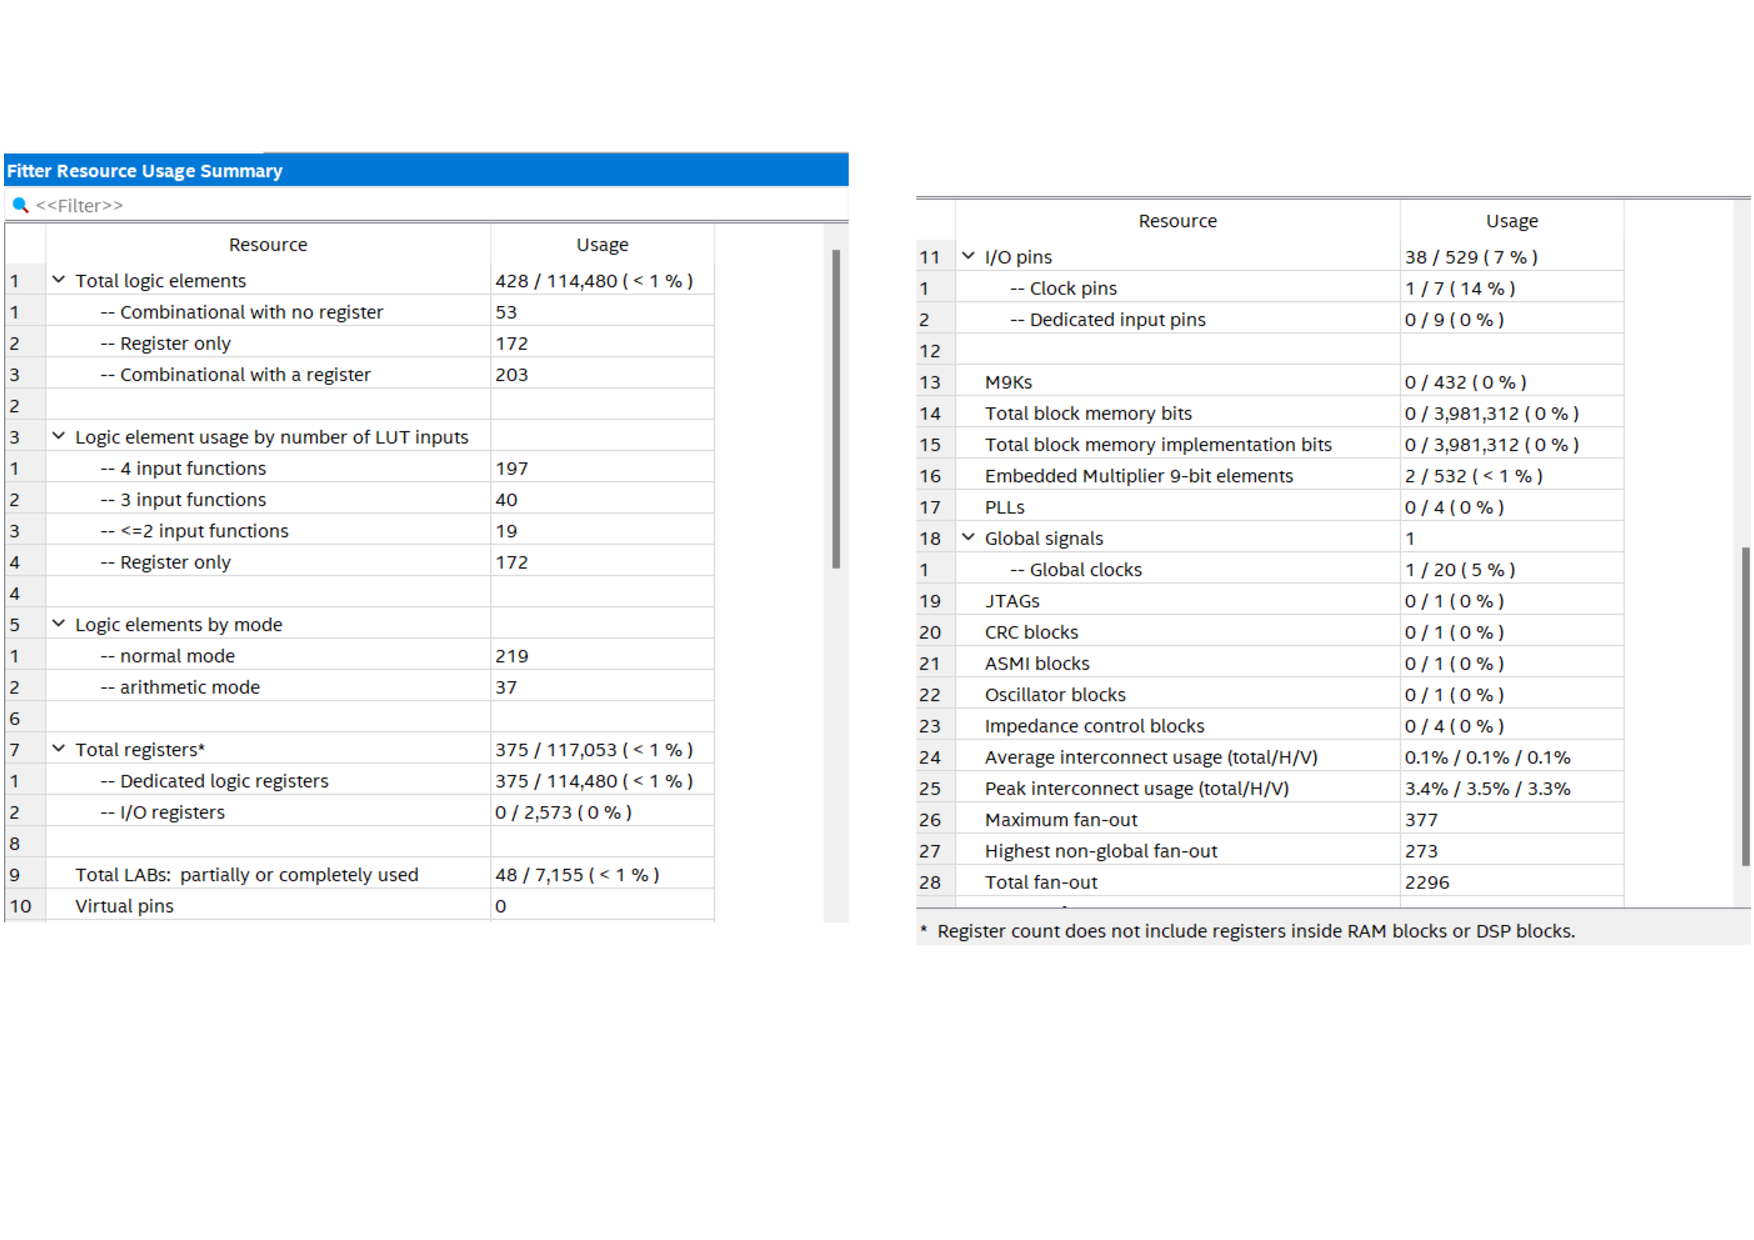
\includegraphics[scale=0.5]{graficosP4/recursos.pdf}
 \caption{Recursos del módulo...} 
 \label{fig:recursos}
 \end{center}
 \end{figure}

 \underline{\textbf{Resultados obtenidos:}}
% captura del resumen de recursos obtenidos con la herramienta Quartus tras la etapa de emplazamiento y rutado (Fitter), que se muestra en el report ``Resource Usage Summary''.

\underline{\textbf{Análisis del resultado:}}
% breve análisis de si los resultados obtenidos

%%%%%%%%%%%%%%%%%%%%%%%%%
%  .d8888b.  888888888  % 
% d88P  Y88b 888        % 
% 888    888 888        % 
% 888    888 8888888b.  % 
% 888    888      "Y88b % 
% 888    888        888 % 
% Y88b  d88P Y88b  d88P % 
%  "Y8888P"   "Y8888P"  % 
%%%%%%%%%%%%%%%%%%%%%%%%%

\subsection{Frecuencia de operación}
%%%%%%%%%%%%%%%%%%%%%%%%%
\begin{enunciado}{}{}

El objetivo de esta sección es que el alumno sea capaz de identificar  el camino crítico del módulo: el que condiciona su frecuencia máxima de funcionamiento.  
\begin{itemize}
    \item Obtenga la frecuencia máxima de operación del módulo implementado en el dispositivo usando la herramienta TimeQuest Timing Analyzer de Quartus e indique dónde se encuentra el camino crítico del circuito. En la tabla aparece un ejemplo de cómo debe indicar el camino crítico: siempre debe indicar desde qué registro se inicia y en qué registro finaliza.
    \item Realice un breve análisis de si es coherente que el camino crítico sea el obtenido por la herramienta TimeQuest o si cree que debería estar en otra parte del circuito.
\end{itemize}

Para realizar el análisis debe tener en cuenta que el camino crítico es el camino entre dos registros con mayor retardo y los retardos en el dispositivo FPGA los producen la lógica combinacional (LUTs) y el rutado. Si un camino tiene más lógica combinacional (más profundidad de lógica: la señal pasa por más LUTs en cascada) generará más retardo debido a la lógica. Si al emplazarse los recursos de un camino concreto (registros y lógica) más separados dentro del chip, esto producirá más retardo por rutado.  

\end{enunciado}

% TABLA DEL INTERFAZ (4 COLUMNAS) %%%%%%%%%%%%%%%%%%%%%%%%
\input{tabla_2col}
% Definir los anchos de columna de la tabla
\def\colUNO{3cm}
\def\colDOS{12cm}
%\def\colTRES{2.0cm}
%\def\colCUATRO{10cm}

\begin{table}[H]
    \caption{Frecuencia de reloj y camino crítico del \emph{comp\_cic}}
    \label{tab:frec_clk}
\gdef\cabecera{\fila{$f_{clk} $ (MHz)}{CAMINO CRÍTICO}}
\noindent\begin{mitabla}
% COMPLETAR FILAS
\fila{}{} 
\end{mitabla}
\end{table}

\underline{\textbf{Análisis del resultado:}}

El camino crítico obtenido es coherente por estas razones ...
%%%%%%%%%%%%%%%%%%%%%%%%%%%%%%%%%%%%%%%%%%%%%%%%%%%%%%%%%%%%%%%%%%%%%%%%%%%%%%%
%  .d8888b.   .d8888b.  % 
% d88P  Y88b d88P  Y88b % 
% 888    888 888        % 
% 888    888 888d888b.  % 
% 888    888 888P "Y88b % 
% 888    888 888    888 % 
% Y88b  d88P Y88b  d88P % 
%  "Y8888P"   "Y8888P"  % 
%%%%%%%%%%%%%%%%%%%%%%%%%


\subsection{Verificación RTL}
%%%%%%%%%%%%%%%%%%%%%%%%%
\begin{enunciado}{}{}%
Resultados de la verificación al excitar el módulo \emph{comp\_cic} con diferentes entradas para demostrar su completo funcionamiento. Solo se incluirá:
\begin{itemize}
\item La lista de las pruebas realizadas que debe coincidir con los casos de test incluidos en el script de simulación de Matlab.
\item Las capturas de las formas de onda y el resumen mostrado en la consola de Modelsim, para un máximo de 2 casos, mostrando claramente el comportamiento del circuito y que no existen errores al compararlo con el modelo de Simulink.  
\end{itemize}
\end{enunciado}
%%%%%%%%%%%%%%%%%%%%%%%%%%%%%%%%%%%%%%%%%%%%%%%%%%%%%%%%%%%%%%%%%%%%%%%%%

El módulo ha funcionado correctamente. Su funcionamiento se ha verificado con las siguientes pruebas:
\begin{enumerate}
    \item 
    \item 
\end{enumerate}

A continuación, se describen dos de los escenarios de test enumerados anteriormente:
\subsubsection{Caso 1: }



\subsubsection{Caso 2:}
%%%%%%%%%%%%%%%%%%%%%%%%%%%%%%%%%%%%%%%%%%%%%%%%%%%%%%%%%%%%%%%%%%%%%%%%%%%%%%%%
%
%  .d8888b.  8888888888 % 
% d88P  Y88b       d88P % 
% 888    888      d88P  % 
% 888    888     d88P   % 
% 888    888  88888888  % 
% 888    888   d88P     % 
% Y88b  d88P  d88P      % 
%  "Y8888P"  d88P       % 
%%%%%%%%%%%%%%%%%%%%%%%%%
%%%%%%%%%%%%%%%%%%%%%%%%%
\subsection{Verificación a nivel de puertas}
%%%%%%%%%%%%%%%%%%%%%%%%%
 \begin{enunciado}{}{}%
Resultados de la verificación \textbf{a nivel de puertas} al excitar el módulo \emph{comp\_cic} con el caso más desfavorable. Incluir la descripción de la prueba realizada y la captura de las formas de onda. Se deberá mostrar claramente el comportamiento del circuito y que no existen errores al compararlo con el modelo de Simulink. 

\end{enunciado}
%%%%%%%%%%%%%%%%%%%%%%%%%%%%%%%%%%%%%%%%%%%%%%%%%%%%%%%%%%%%%%%%%%%%%%%%
%%%%%%%%%%%%%%%%%%%%%%%%%%%%%%%%%%%%%%%%%%%%%%%%%%%%%%%%%%%%%%%%%%%%%%%%%
%%%%%%%%%%%%%%%%%%%%%%%%%
%  .d8888b.   .d8888b.  % 
% d88P  Y88b d88P  Y88b % 
% 888    888 Y88b. d88P % 
% 888    888  "Y88888"  % 
% 888    888 .d8P""Y8b. % 
% 888    888 888    888 % 
% Y88b  d88P Y88b  d88P % 
%  "Y8888P"   "Y8888P"  % 
%%%%%%%%%%%%%%%%%%%%%%%%%

\section{Conclusiones}
%%%%%%%%%%%%%%%%%%%%%%%%%
\begin{enunciado}{}{}%
Conclusiones de la práctica P4\_1. Valore el grado de cumplimiento de los objetivos de la práctica. Haga un breve análisis de si los resultados obtenidos de área y frecuencia máxima son coherentes.  

\end{enunciado}


%%%%%%%%%%%%%%%%%%%%%%%%%%%%%%%%%%%%%%%%%%%%%%%%%%%%%%%%%%%%%%%%%%%%%%%%
%%%%%%%%%%%%%%%%%%%%%%%%%%%%%%%%%%%%%%%%%%%%%%%%%%%%%%%%%%%%%%%%%%%%%%%%%
%%%%%%%%%%%%%%%%%%%%%%%%%
%  .d8888b.   .d8888b.  % 
% d88P  Y88b d88P  Y88b % 
% 888    888 Y88b. d88P % 
% 888    888  "Y88888"  % 
% 888    888 .d8P""Y8b. % 
% 888    888 888    888 % 
% Y88b  d88P Y88b  d88P % 
%  "Y8888P"   "Y8888P"  % 
%%%%%%%%%%%%%%%%%%%%%%%%%
\section{P4\_2: Filtro compensador del DAC}
\subsection{Diseño de la estructura del filtro compensador del DAC}
\begin{enunciado}{}{}%
Incluya un dibujo de la estructura del filtro paralelo a implementar, de manera que aproveche la simetría de los coeficientes y realice los multiplicadores cableados. Marque claramente los puntos en los que segmentará para obtener la máxima velocidad del circuito.
\end{enunciado}

%%%%%%%%%%%%%%%%%%%%%%%%%
%  .d8888b.   .d8888b.  % 
% d88P  Y88b d88P  Y88b % 
% 888    888 888    888 % 
% 888    888 Y88b. d888 % 
% 888    888  "Y888P888 % 
% 888    888        888 % 
% Y88b  d88P Y88b  d88P % 
%  "Y8888P"   "Y8888P"  % 
%%%%%%%%%%%%%%%%%%%%%%%%%
\subsection{Análisis de la cuantificación de la ruta de datos}
\begin{enunciado}{}{}%
Indique, sobre el dibujo de la estructura del filtro, la cuantificación a la salida de cada operador incluido en el filtro.
\end{enunciado}

%%%%%%%%%%%%%%%%%%%%%%%%%
%  d888     .d8888b.   % 
% d8888    d88P  Y88b  % 
%   888    888    888  % 
%   888    888    888  % 
%   888    888    888  % 
%   888    888    888  % 
%   888    Y88b  d88P  % 
% 8888888  "Y8888P"   % 
%%%%%%%%%%%%%%%%%%%%%%%%%
\subsection{Interfaz}

\begin{enunciado}{}{}%
Incluir la tabla para definir el interfaz del módulo \emph{comp\_dac} implementado, sus formatos y sus parámetros. 
\end{enunciado}
% TABLA DEL INTERFAZ (4 COLUMNAS) %%%%%%%%%%%%%%%%%%%%%%%%
\input{tabla_4col}
% Definir los anchos de columna de la tabla
\def\colUNO{2cm}
\def\colDOS{1cm}
\def\colTRES{2.0cm}
\def\colCUATRO{10cm}

\begin{table}[H]
    \caption{Interfaz del módulo  \emph{comp\_dac}}
    \label{tab:interfaz}
\gdef\cabecera{\fila{NOMBRE}{TIPO}{FORMATO}{DESCRIPCIÓN}}
\noindent\begin{mitabla}
% COMPLETAR FILAS. AÑADA LAS QUE NECESITE
\fila{}{}{}{} 
\fila{}{}{}{} 
\fila{}{}{}{} 
\fila{}{}{}{} 
\fila{}{}{}{} 
\fila{}{}{}{} 
\fila{}{}{}{} 
\fila{}{}{}{} 
\fila{}{}{}{} 
\fila{}{}{}{} 
\end{mitabla}
\end{table}


%%%%%%%%%%%%%%%%%%%%%%
%   d888     d888   % 
%  d8888    d8888   % 
%    888      888   % 
%    888      888   % 
%    888      888   % 
%    888      888   % 
%    888      888   % 
%  8888888  8888888 % 
%%%%%%%%%%%%%%%%%%%%%%
\subsection{Recursos hardware}
\begin{enunciado}{}{}%
El objetivo de esta sección es que el alumno sea capaz de identificar si los recursos obtenidos en la implementación son coherentes con los esperables para el circuito realizado.

Se deberán incluir las siguientes partes: 
\begin{itemize}
\item \textbf{Estimación de recursos:} Un breve desglose de la estimación de recursos  del dispositivo FPGA que se requieren para implementar el módulo, indicando la cantidad de recursos asignados a cada bloque de su diseño. El resultado final se mostrará en una tabla. En esta práctica solo hay que indicar el número de LEs en modo aritmético y los FFs. 

\item \textbf{Resultados obtenidos:} Una captura del resumen de recursos obtenidos con la herramienta Quartus tras la etapa de emplazamiento y rutado (Fitter), que se muestra en el report ``Resource Usage Summary''.  

\item \textbf{Análisis del resultado:} Un breve análisis de si los resultados obtenidos son coherentes con la estimación de recursos realizada. El análisis se realizará en base a la comparación entre lo estimado y obtenido en Quartus. Si hay muchas discrepancias con los recursos obtenidos, indicar razonadamente las causas de dicha discrepancia.
\end{itemize}

\end{enunciado}
%%%%%%%%%%%%%%%%%%%%%%%%%%%%%%%%%%%%%%%%%%%%%%%%%%%%%%%%%%%%%%%%%%%%%%%%%
Los recursos hardware necesarios para implementar el bloque CIC son los siguientes:
\begin{itemize}
\item \textbf{FFs:} 


\item \textbf{LEs aritméticos:} 

\end{itemize}

A continuación se muestra la tabla con el resumen de los recursos: 

% TABLA DEL INTERFAZ %%%%%%%%%%%%%%%%%%%%%%%%
\input{tabla_3col}
% Definir los anchos de columna de la tabla
\def\colUNO{5.5 cm}
\def\colDOS{5 cm}
\def\colTRES{5 cm}
%\def\colCUATRO{10cm}

\begin{table}[H]
\centering
    \caption{Recursos hardware}
    \label{tab:recursos_HW}
\gdef\cabecera{\fila{RECURSO}{NÚMERO OBTENIDO}{NÚMERO ESTIMADO}}
\noindent\begin{mitabla}
% COMPLETAR FILAS
\fila{FFs}{}{}  
\fila{LEs-aritméticos}{}{}  
\end{mitabla}
\end{table}

A continuación se muestra la captura realizada de los recursos obtenidos tras la etapa de emplazamiento y rutado (\textit{Fitter}) en el ``\textit{ Resource Usage Summary}'': 

  \begin{center}
 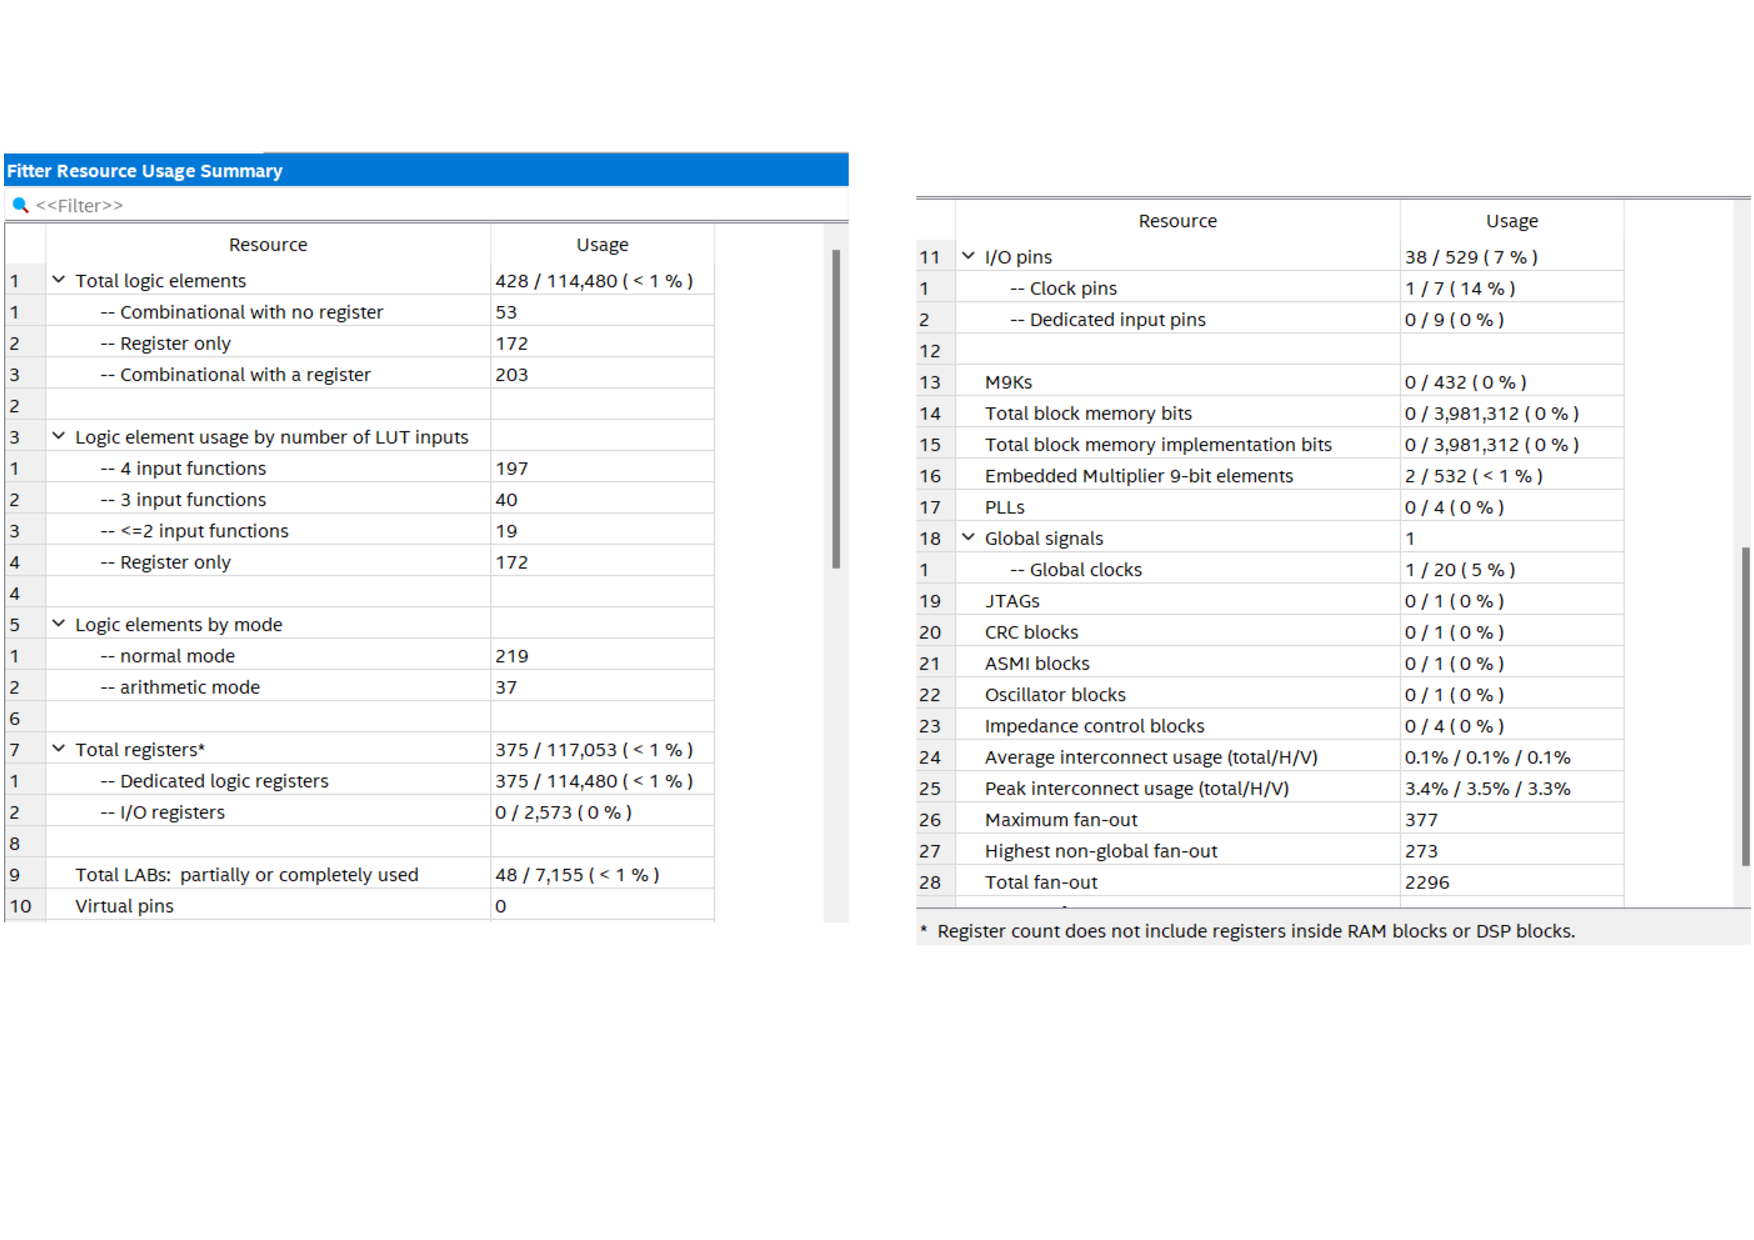
\includegraphics[scale=0.5]{graficosP4/recursos.pdf}
 \end{center}
%%%%%%%%%%%%%%%%%%%%%%%%%%%%%%%%%%%%%%%%%%%%%%%%%%%%%%%%%%%%%%%%%%%%%%%%%

%%%%%%%%%%%%%%%%%%%%%%%%
%   d888     .d8888b.  % 
%  d8888    d88P  Y88b % 
%    888           888 %  
%    888         .d88P %   
%    888     .od888P"  %      
%    888    d88P"      %       
%    888    888"       %     
%  8888888  888888888  % 
%%%%%%%%%%%%%%%%%%%%%%%%% 
\subsection{Frecuencia de operación}
%%%%%%%%%%%%%%%%%%%%%%%%%
\begin{enunciado}{}{}

El objetivo de esta sección es que el alumno sea capaz de identificar  el camino crítico del módulo: el que condiciona su frecuencia máxima de funcionamiento.  
\begin{itemize}
    \item Obtenga la frecuencia máxima de operación del módulo implementado en el dispositivo usando la herramienta TimeQuest Timing Analyzer de Quartus e indique dónde se encuentra el camino crítico del circuito. En la tabla aparece un ejemplo de cómo debe indicar el camino crítico: siempre debe indicar desde qué registro se inicia y en qué registro finaliza.
    \item Realice un breve análisis de si es coherente que el camino crítico sea el obtenido por la herramienta TimeQuest o si cree que debería estar en otra parte del circuito.
\end{itemize}

Para realizar el análisis debe tener en cuenta que el camino crítico es el camino entre dos registros con mayor retardo y los retardos en el dispositivo FPGA los producen la lógica combinacional (LUTs) y el rutado. Si un camino tiene más lógica combinacional (más profundidad de lógica: la señal pasa por más LUTs en cascada) generará más retardo debido a la lógica. Si al emplazarse los recursos de un camino concreto (registros y lógica) más separados dentro del chip, esto producirá más retardo por rutado.  

\end{enunciado}

% TABLA DE frecuencia %%%%%%%%%%%%%%%%%%%%%%%%
\input{tabla_2col}
% Definir los anchos de columna de la tabla
\def\colUNO{3cm}
\def\colDOS{12cm}
%\def\colTRES{2.0cm}
%\def\colCUATRO{10cm}

\begin{table}[H]
    \caption{Frecuencia de reloj y camino crítico del \emph{comp\_dac}}
    \label{tab:frec_clk}
\gdef\cabecera{\fila{$f_{clk} $ (MHz)}{CAMINO CRÍTICO}}
\noindent\begin{mitabla}
% COMPLETAR FILAS
\fila{}{} 
\end{mitabla}
\end{table}

\underline{\textbf{Análisis del resultado:}}

El camino crítico obtenido es coherente por estas razones ...
%%%%%%%%%%%%%%%%%%%%%%%%% 
%   d888      .d8888b.  % 
%  d8888     d88P  Y88b % 
%    888          .d88P % 
%    888         8888"  % 
%    888          "Y8b. % 
%    888     888    888 % 
%    888     Y88b  d88P % 
%  8888888   "Y8888P"  % 
%%%%%%%%%%%%%%%%%%%%%%%%% 
\subsection{Verificación RTL}
%%%%%%%%%%%%%%%%%%%%%%%%%
\begin{enunciado}{}{}%
Resultados de la verificación (RTL) al excitar el módulo \emph{comp\_dac} con el estímulo más desfavorable, mostrando claramente el comportamiento del circuito y que no existen errores al compararlo con el modelo de Simulink.  

\end{enunciado}
%%%%%%%%%%%%%%%%%%%%%%%%%%%%%%%%%%%%%%%%%%%%%%%%%%%%%%%%%%%%%%%%%%%%%%%%%

El módulo ha funcionado correctamente. Su funcionamiento se ha verificado con la siguiente prueba:
\begin{enumerate}
    \item 
\end{enumerate}

A continuación, se describe el escenario de test:
\subsubsection{Caso 1: }

%   \begin{center}
%   \includegraphics[width=19cm]{XXXXX.png}
%   \end{center}


%%%%%%%%%%%%%%%%%%%%%%%%%
%   d888         d8888  % 
%  d8888        d8P888  % 
%    888       d8P 888  % 
%    888      d8P  888  % 
%    888     d88   888  % 
%    888     8888888888 % 
%    888           888  % 
%  8888888         888  % 
%%%%%%%%%%%%%%%%%%%%%%%%%

\section{Conclusiones}
%%%%%%%%%%%%%%%%%%%%%%%%%
\begin{enunciado}{}{}%
Conclusiones de la práctica P4\_2. Valore el grado de cumplimiento de los objetivos de la práctica. Haga un breve análisis de si los resultados obtenidos de área y frecuencia máxima son coherentes.  

Destaque los problemas encontrados durante el desarrollo de la práctica y cómo los ha resuelto.
\end{enunciado}


\section{Ficheros entregados}
%%%%%%%%%%%%%%%%%%%%%%%%%
\begin{enunciado}{}{}%
Lea el documento \href{https://gised.webs.upv.es/pds_fpga/PDS_FPGA_practicas.pdf} {desarrollo y entrega de prácticas}  e indique cómo se han nombrado los ficheros que se indican en la tabla.

\end{enunciado}
%%%%%%%%%%%%%%%%%%%%%%%%%%%%%%%%%%%%%%%%%%%%%%%%%%%%%%%%%%%%%%%%%%%%%%%%%

Los autores de la memoria confirman que han entregado los siguientes ficheros, siguiendo las pautas indicadas:
% TABLA DE PARÁMTROS (2 COLUMNAS) %%%%%%%%%%%%%%%%%%%%%%%%
\input{tabla_2col}
% Definir los anchos de columna de la tabla
\def\colUNO{10cm}
\def\colDOS{4cm}

\begin{table}[H]
    \centering
    %\caption{Entregables de la práctica E1}
    \label{tab:entregables}
\gdef\cabecera{\fila{FICHERO}{NOMBRE}}
\noindent\begin{mitabla}
% COMPLETAR FILAS. AÑADA LAS QUE NECESITE
\fila{Memoria de prácticas}{Memoria\_P4\_Gx.pdf}
\fila{Entrega de los ficheros de prácticas}{Proy\_sim\_P4\_Gx.zip}
\fila{Proyecto Modelsim P4\_1}{}
\fila{Fichero .do}{*.do}
\fila{Fichero .tcl}{*.tcl}
\fila{Proyecto Quartus P4\_1}{}
\fila{Proyecto Modelsim P4\_2}{}
\fila{Fichero .do}{*.do}
\fila{Fichero .tcl}{*.tcl}
\fila{Proyecto Quartus P4\_2}{}
\end{mitabla}
\end{table}


\section{ANEXO 1: Código HDL de los módulos implementados en P4\_1}

%%%%%%%%%%%%%%%%%%%%%%%%%
\begin{enunciado}{}{}%
Incluir el código Verilog de los módulos de la práctica. El código debe seguir las pautas indicadas en el documento  \href{https://gised.webs.upv.es/pds_fpga/PDS_FPGA_practicas.pdf} {desarrollo y entrega de prácticas}. 
\end{enunciado}
%%%%%%%%%%%%%%%%%%%%%%%%%%%%%%%%%%%%%%%%%%%%%%%%%%%%%%%%%%%%%%%%%%%%%%%%%

\begin{minted}[fontsize=\footnotesize,obeytabs=true,tabsize=2]{verilog}
module comp_cic
#(  parameter Win=16,    // Input Wordlength 
    parameter Wcoef = XX,   // Coefficients Wordlength
    parameter Wout = 18,  // Output wordlength
    parameter Ng = XX,    // Filter growth
    parameter Num_coef=17)   // Coefficients number
(
 input  signed [Win-1:0] id_data_filter, // Input S[16 15]
 input  clk, 
 input ic_val_data,
 input ic_rst,
 output signed [Wout-1:0] od_data_filter, // S[18 15]
 output oc_val_data); 
/* DECLARACIONES ----------------------- */

/* DESCRIPCION ------------------------- */	

/* ASIGNACION SALIDAS ------------------ */

endmodule 
\end{minted}




\section{ANEXO 2: Código HDL del banco de pruebas comp\_cic\_tsb}
%%%%%%%%%%%%%%%%%%%%%%%%%
\begin{enunciado}{}{}%
Incluir el código Verilog del banco de pruebas realizado.
\end{enunciado}
%%%%%%%%%%%%%%%%%%%%%%%%%%%%%%%%%%%%%%%%%%%%%%%%%%%%%%%%%%%%%%%%%%%%%%%%%

\begin{minted}[fontsize=\footnotesize,obeytabs=true,tabsize=2]{verilog}
`timescale 1ns/1ps

module comp_cic_tsb();


endmodule 

\end{minted}
\section{ANEXO 3: Código HDL de los módulos implementados en P4\_2}

%%%%%%%%%%%%%%%%%%%%%%%%%
\begin{enunciado}{}{}%
Incluir el código Verilog de los módulos de la práctica. El código debe seguir las pautas indicadas en el documento  \href{https://gised.webs.upv.es/pds_fpga/PDS_FPGA_practicas.pdf} {desarrollo y entrega de prácticas}. 
\end{enunciado}
%%%%%%%%%%%%%%%%%%%%%%%%%%%%%%%%%%%%%%%%%%%%%%%%%%%%%%%%%%%%%%%%%%%%%%%%%

\begin{minted}[fontsize=\footnotesize,obeytabs=true,tabsize=2]{verilog}
module comp_dac
#(parameter Win=16,  // Module input wordlength
parameter Wout = 14)// Module output wordlength

(input signed [Win-1:0] id_data, // S[Win, Win-1]
input ic_val_data, 
input clk,
output signed [Wout-1:0 ] od_data,// S[Wout, Wout-1]
output oc_val_data); 
	
/* DECLARACIONES ----------------------- */

/* DESCRIPCION ------------------------- */	

/* ASIGNACION SALIDAS ------------------ */

endmodule 
\end{minted}




\section{ANEXO 4: Código HDL del banco de pruebas comp\_dac\_tsb}
%%%%%%%%%%%%%%%%%%%%%%%%%
\begin{enunciado}{}{}%
Incluir el código Verilog del banco de pruebas realizado.
\end{enunciado}
%%%%%%%%%%%%%%%%%%%%%%%%%%%%%%%%%%%%%%%%%%%%%%%%%%%%%%%%%%%%%%%%%%%%%%%%%

\begin{minted}[fontsize=\footnotesize,obeytabs=true,tabsize=2]{verilog}
`timescale 1ns/1ps

module comp_dac_tsb();


endmodule 

\end{minted}



\end{document}